%Author: Martiano Jimenez
%Date: 30.December.2024

\documentclass[11pt]{beamer}
\usetheme{Darmstadt}
\usepackage[utf8]{inputenc}
\usepackage[spanish]{babel}
\usepackage{amsmath}
\usepackage{amsfonts}
\usepackage{amssymb}
\usepackage{graphicx}
\author{Ing. Mariano Jim\'enez Brenes}
\title
{
E2025C2-G01-ELECTRÓNICA DIGITAL Y SEMICONDUCTORES.\linebreak
Mapas de Karnaugh.
}
%\setbeamercovered{transparent} 
%\setbeamertemplate{navigation symbols}{} 
\logo{
\includegraphics[height=0.75cm]{./images/castrocarazo.eps}\vspace{5pt}} 
\institute{
Universidad Castro Carazo\linebreak
T\'ecnico En Semiconductores
} 
\date{Mi\'ercoles 21.Mayo.2025} 
%\subject{} 
\begin{document}

\begin{frame}
\maketitle 
\end{frame}

% Remove logo from the next slides
\logo{}

\begin{frame}
\frametitle{Contenido}
\tableofcontents
\end{frame}


\section{Mapas K}
	\subsection{Mapa K de 2 variables}
	\begin{frame}{Mapa K de 2 variables}
	\frametitle{Mapa K de 2 variables}

	\end{frame}

	\subsection{Mapa K de 3 variables}
	\begin{frame}{Mapa K de 3 variables}
	\frametitle{Mapa K de 3 variables}

	\end{frame}

	\subsection{Mapa K de 4 variables}
	\begin{frame}{Mapa K de 4 variables}
	\frametitle{Mapa K de 4 variables}

	\end{frame}

\section{Ejemplos}

	\subsection{Mapa K de 3 variables}
	\begin{frame}{Mapa K de 3 variables}
	\frametitle{Mapa K de 3 variables}

\section{Ejercicios}
\begin{frame}{Ejercicios}
\frametitle{Ejercicios}
\begin{figure}[h]
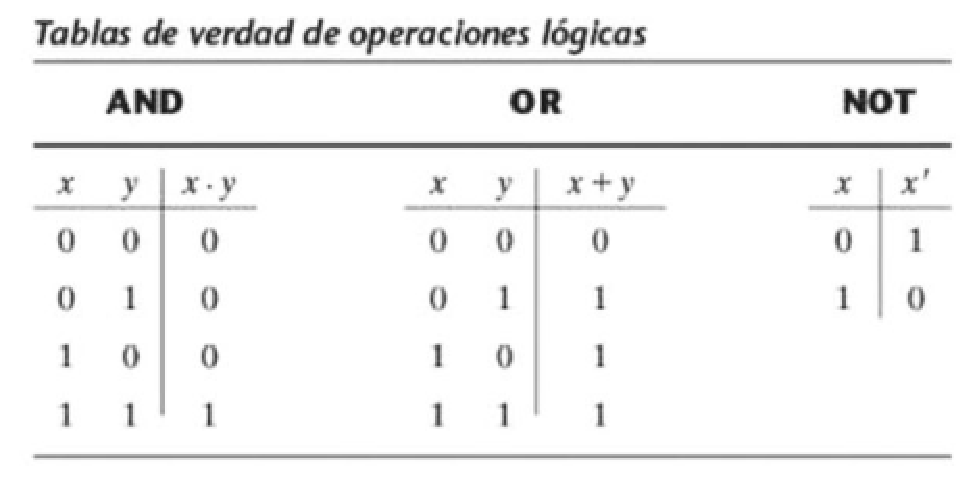
\includegraphics[height=3.0cm]{./images/tt.eps}\vspace{1pt}
\end{figure}
\end{frame}

\section{Actividades Asincr\'onicas}
\begin{frame}
\frametitle{Actividades Asincr\'onicas}

\end{frame}

\section{Bibliograf\'ia}
\begin{frame}
	\frametitle{Bibliograf\'ia}
	\begin{itemize}
		\item Morris, M., y Ciletti, M. Diseño Digital, Cap. 3, pág. 73-96.
		\item Argüello D. M, Pérez, S., y Facchini, H. Arquitectura de computadoras, Cap.3, pág. 64-79.
		\end{itemize}
\end{frame}

\end{document}